\section{Application Scenarios}
\label{sec:caseStudy}
% \shusen{A full case study that driven by the visualization task and the question associated with them}
%In this section, we discuss application scenarios, in which the domain experts utilize the 
To better illustrate how the proposed perturbation-driven exploration tool helps the domain experts interpret the neural network model, we present five application scenarios gathered by the domain experts who integrated the proposed tool into their model analysis workflow.

\begin{figure}[htbp]
\centering
\vspace{-2mm}
 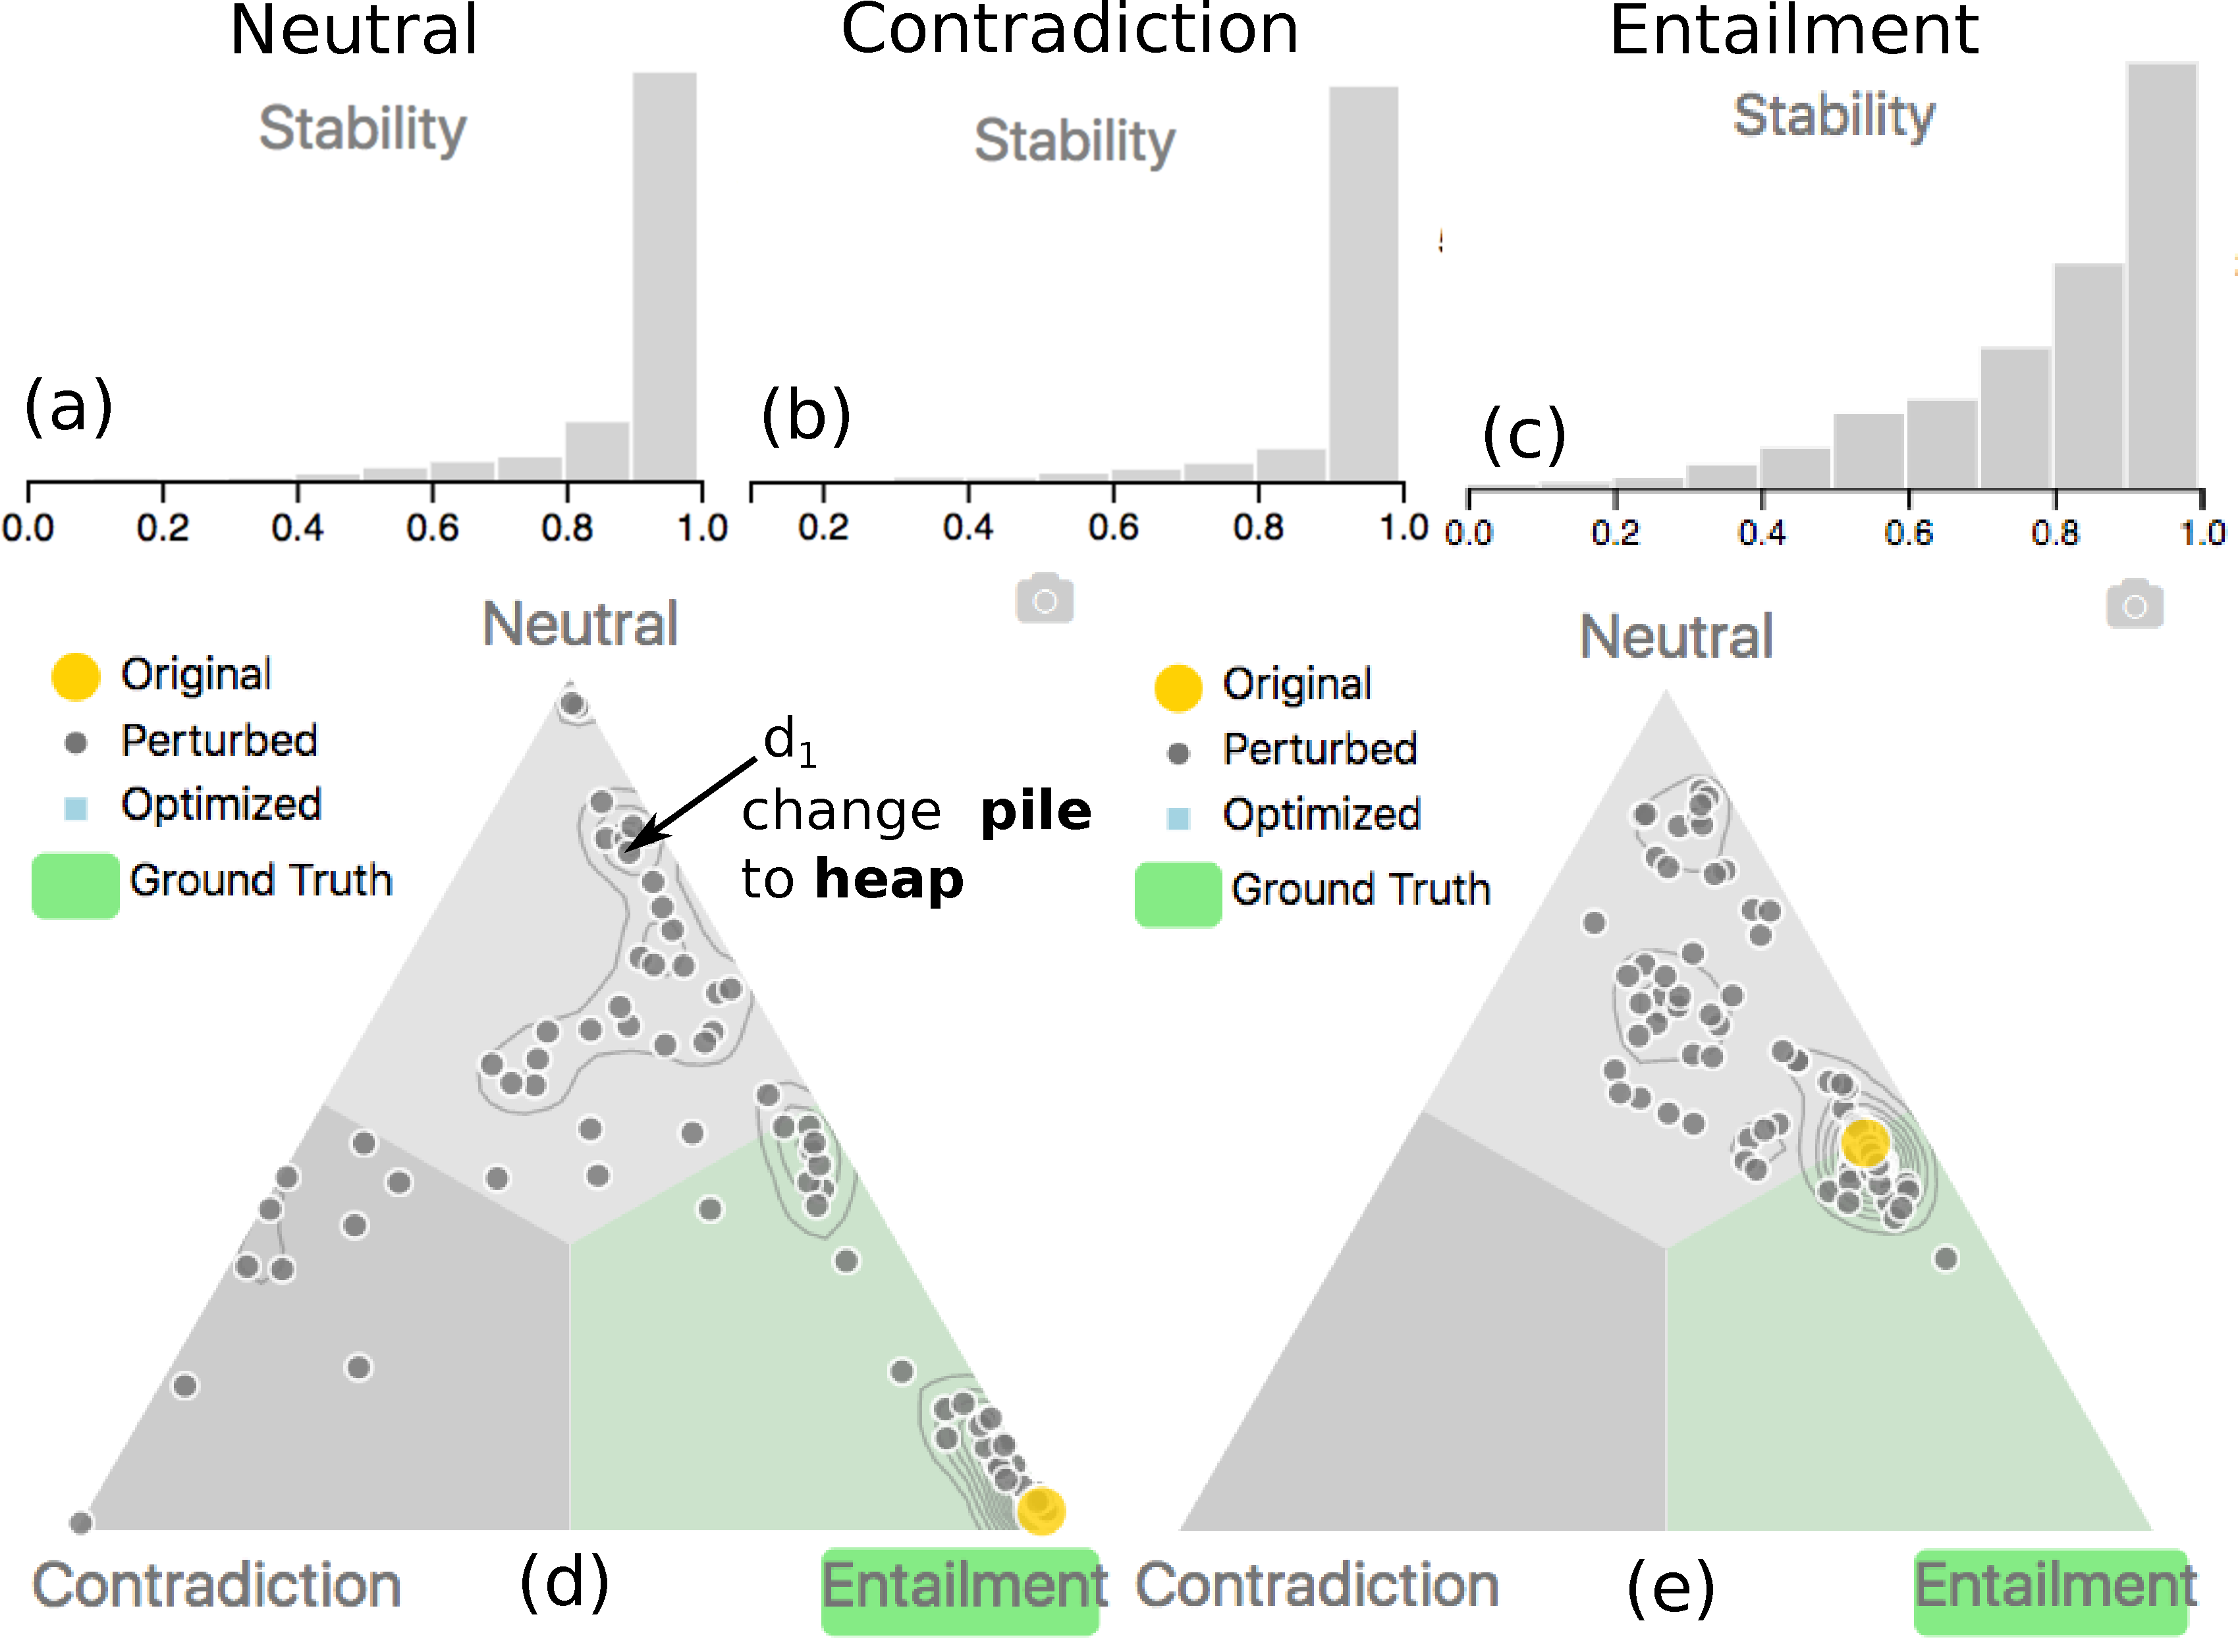
\includegraphics[width=1.0\linewidth]{predictStability}
 \caption{
Prediction stability assessment. Isolate unstable one
 }
\label{fig:pipelineView}
\end{figure}

\subsection{Scenario 1: Assess the Model Prediction Stability}
Utilize input sentence perturbation to assess the overall stability of the prediction

\subsection{Scenario 1: Interpreting Decision Making Process}
Understand how the model arrive at the prediction is the first step  only essential for evaluating the model performance but also necessary for hypothesizing improvement strategies.
%
The three stages (encoder, attention, classifier) of the model work in synergy to produce the correct prediction.
%
%One of the essential task for can be made in either of these stages.
% \shusen{difference in sensitivity among entail natural and contradict relationships}
% the generate the correct prediction for the wrong reason

\subsection{Scenario 2: What Does It Take to Correct a Wrong Prediction?}
In the previous section, we discussed how we can use forward prediction



\subsection{Scenario 4: Handcraft Example Analysis}
Well-known tough examples, such as the Facebook IPO example discussed in Section~\ref{sec:background}.

\subsection{Scenario 5: Explore Relationship Between Grammar and Attention}
Can attention capture grammar structure? Is 
%\subsection{Is the Prediction Stable?}
%\subsection{Where Are the Mistakes?}
%\subsection{How Attention Affect the Prediction?}
%\subsection{What Does It Take to Change the Prediction?}
%\subsection{Is Attention All You Need?}
